\section{Experiments}
\subsection{Code optimisations}
For a first experiment, a second version of the code was written in order to utilise more of the faster cache. Below are the timings for each version on different optimisation flags.
\begin{center}
    \begin{tabular}{|c|c|c|c|c|}
        \hline
        Version & -O0 & -O3 & -Ofast & -O3 -Ofast -march=native\\
        \hline
        1 & 11.632 & 5.521 & 5.318 & 5.051\\
        \hline
        2 & 18.547 & 4.857 & 4.796 & 4.503\\
        \hline
    \end{tabular}
\end{center}
As can be seen, the optimised code runs faster for all flags aside from -O0. This optimisation can be viewed in the appendix.

The next experiment was to test the how the code performed upon increasing the size of the matrix A. Below is a graphic showing how Version 1 compares with Version 2 with the optimised flags -O3, -Ofast and -march=native on both my laptop and the machines at the university.

\begin{figure}[htb]
    \begin{center}
        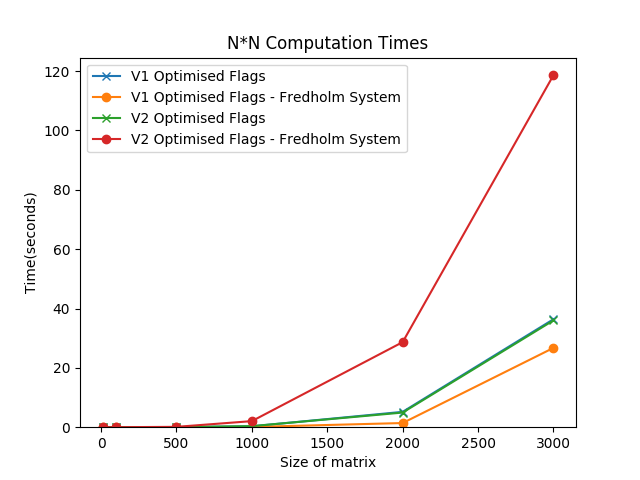
\includegraphics[width=8cm]{../images/NN_comp_times.png}
        \caption{Computation Times on an N*N matrix}
    \end{center}
\end{figure}

We chose to extend the size of the matrix to something that would compute for a reasonable length of time so that we may be able to ascertain what happens as a general trend.

From the graphics, we can see that up to around a matrix size of $N = 2000$, everything runs quickly aside from Version 2 with the Fredholm system. The reason behind this is unknown at this moment in time. Computation times start to get much slower at $N = 3000$.
\subsection{Parallelisation}
Another experiment that I wanted to test was the effectiveness of using OpenMP within my code. I inserted a parallelisation above the for loop to compute the lower matrix.

\begin{figure}[htb]
    \begin{center}
        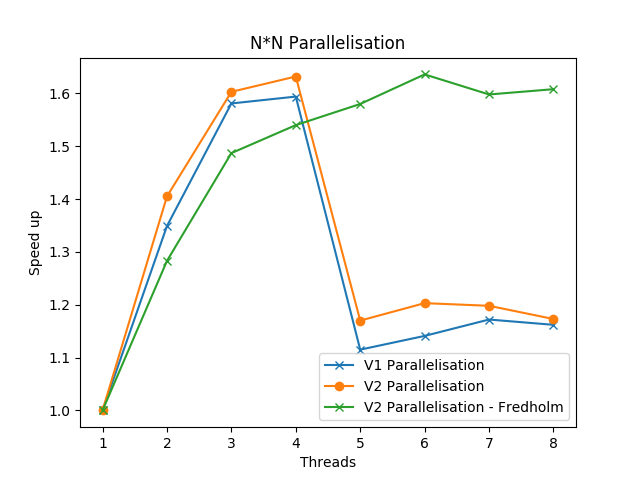
\includegraphics[width=8cm]{../images/NN_speedup.png}
        \caption{Speed up graphic: OpenMP}
    \end{center}
\end{figure}

To test this, I increased the number of threads that I wanted to run the code on each time. As we can see from the graphic, all versions and systems increased with speed up, up until the fourth thread, at which point, my system slowed down again. This could be due to the fact that my laptop runs with four cores and that the system at the university runs with eight. The systems at the university appear to level off in a much smoother manner. However, we can see that the speed up times are nothing near what I would like. So there would appear to be a great deal of optimisations to do.
\subsection{Unsuccessful Optimisations}
I had some other optimisations that I tried but were unsuccessful. First of all, I tried to use some loop unrolling on some of the for loops to get some performance benefit. Unfortunately, this resulted in some failed output with core dumping. There could have been an issue with the number of computations to do and that this being a number not divisible by the number of loops unrolled. Further to this, I also tried to add -funroll-loops into the Makefile. Upon running this, I found no performance benefit, so excluded this.

Another attempt at optimisation was to make use of the OpenMP parallelisation option above other for loops. When trying this, I found that adding this to some loops increased computation time. This could be due to the loop trying to access different elements of the array that may not be accessible at that moment in time, so the output matrix gives incorrect results.
